% !TeX root = ../../../geos_mpm_manual.tex
\section{Contact options: fields, normals, gap closure, and overlap control}
\label{sec:contact-surface-detection-spacing}
\label{sec:contact-options}
\index{contact!options}
\index{contact!multi-field}
\index{damage-field gradient}
\index{DFG}
\index{contact!normal}
\index{contact!gap closure}
\index{overdensification}

This section documents the solver-side contact machinery.  It intentionally focuses on the internal fields, algorithms, and option-dependent branches.  User-facing input controls are collected in Section~\ref{sec:pfw-boundary-controls}, and the generated attribute inventory in Appendix~\ref{app:solver-attributes} should be used as the authoritative list of currently registered solver keys.  At the algorithmic level, GEOS-MPM contact follows the multi-velocity-field MPM contact family of Bardenhagen, Brackbill, Sulsky, Guilkey, and coworkers \cite{bardenhagen2000granular,bardenhagen2001contact}.  GEOS-MPM then provides several complementary ways to create the contact fields and contact geometry.  Prescribed multi-field contact uses user-assigned particle groups.  Dynamic same-material fracture/contact uses the damage-field-gradient, or DFG, partition of Homel and Herbold \cite{homel2016dfg}.  Logistic-regression contact reconstructs a separating plane from the local point cloud following Nairn, Hammerquist, and Smith \cite{nairn2020contact}.  In addition, the cohesive-zone implementation described in Section~\ref{sec:cohesive-zone-implementation} can provide exact surface-contact data: stored surface positions and normals define the gap plane for curved boundaries, so the contact normal and gap are not forced to follow stair-step particle domains.  This removes the particle-domain stair-step discretization error in the contact geometry for those cohesive-zone-derived surfaces, while the usual grid-transfer, time-integration, and constitutive-discretization errors remain \cite{crook2025cohesive}.  The experimental weak-trace projection described in Section~\ref{sec:weak-trace-implementation} uses the same multi-field and surface-geometry data paths, but it is a bonded-interface projection rather than a separable contact law.

\subsection{Nodal contact state and activation}
\label{subsec:contact-state-activation}
\index{contact!activation}

GEOS-MPM treats material contact as a nodal, pairwise correction between velocity fields.  At a grid node $I$, each velocity field $\alpha$ carries field-specific mass $m_{I\alpha}$, momentum $\mathbf{q}_{I\alpha}$, velocity $\mathbf{v}_{I\alpha}$, material volume $V_{I\alpha}$, damage summaries, center of mass or center of volume, and surface geometry fields such as $\mathbf{n}_{I\alpha}$ and $\mathbf{x}^{s}_{I\alpha}$.  Contact is active only when both the global contact switch is on and the run actually has multiple velocity fields or contact-wall boundaries,
\begin{equation}
  \texttt{hasContact} =
  \left(N_{\mathrm{fields}}>1\right)
  \lor
  \left(\exists\,\hbox{face with }\texttt{boundaryConditionTypes}=\texttt{Contact}\right).
\end{equation}
For material-material contact, the contact update loops over each nodal pair $(A,B)$ with $A<B$, checks that both field masses exceed the small-mass cutoff, constructs an effective pair normal $\hat{\mathbf{n}}_{AB}$, evaluates whether the pair is separable, and then applies equal-and-opposite force or impulse corrections.  The ordinary lumped update uses a force form, while the FMPM path uses the same kinematics in impulse form so that the cumulative contact impulse can be used by the incremental full-mass-matrix correction.

\begin{lstlisting}[language=Python,caption={Solver-level material contact loop.}]
for node I:
    for fields A < B:
        if m[I,A] <= smallMass or m[I,B] <= smallMass:
            continue
        nAB = pair_normal(I,A,B, contactNormalType)
        if norm(nAB) is tiny:
            nAB = n[I,A]
        if planeStrain:
            nAB.z = 0
        nAB = normalize(nAB)
        separable = evaluate_separability(I,A,B)
        apply_pairwise_contact(I,A,B,nAB,separable,
                               contactGapCorrection,
                               overlapCorrection,
                               frictionCoefficientTable)
\end{lstlisting}

\subsection{Prescribed multi-field contact groups}
\label{subsec:prescribed-multifield-contact}
\index{contact!prescribed groups}
\index{particleGroup}

A prescribed multi-field contact calculation begins with the particle field \texttt{particleGroup}.  During initialization, the solver finds the maximum group index over all active particle subregions and sets
\begin{equation}
  N_g = 1 + \max_p g_p,
\end{equation}
where $g_p$ is the stored particle group.  A protective check rejects cases with more than 100 prescribed groups, which is intended to catch accidental large group identifiers before they create excessive nodal storage.  If DFG partitioning is disabled, the field index is simply
\begin{equation}
  \alpha = g_p, \qquad N_{\mathrm{fields}}=N_g.
\end{equation}
Thus, particles in different groups scatter mass, momentum, internal force, damage summaries, and surface fields to different velocity fields at the same grid node.  Pairwise contact between fields with different group indices is considered a prescribed material-material interface.  The same prescribed-group separation is currently the simplest way to provide the two velocity fields used by the experimental weak-trace projection in Section~\ref{sec:weak-trace-implementation}.  In that mode, the selected group pair is coupled by trace velocity compatibility at a prescribed interface point rather than by the ordinary nodal contact impulse.  The pairwise friction coefficient is taken from \texttt{frictionCoefficientTable} by reducing the field indices modulo the prescribed group count,
\begin{equation}
  \mu_{AB}=\mu_{A\bmod N_g,\,B\bmod N_g}.
\end{equation}
This modulo rule is important when DFG is also enabled, because it keeps friction material-pair-based even after each prescribed group is split into damage-side subfields.

\begin{figure}[htbp]
  \centering
  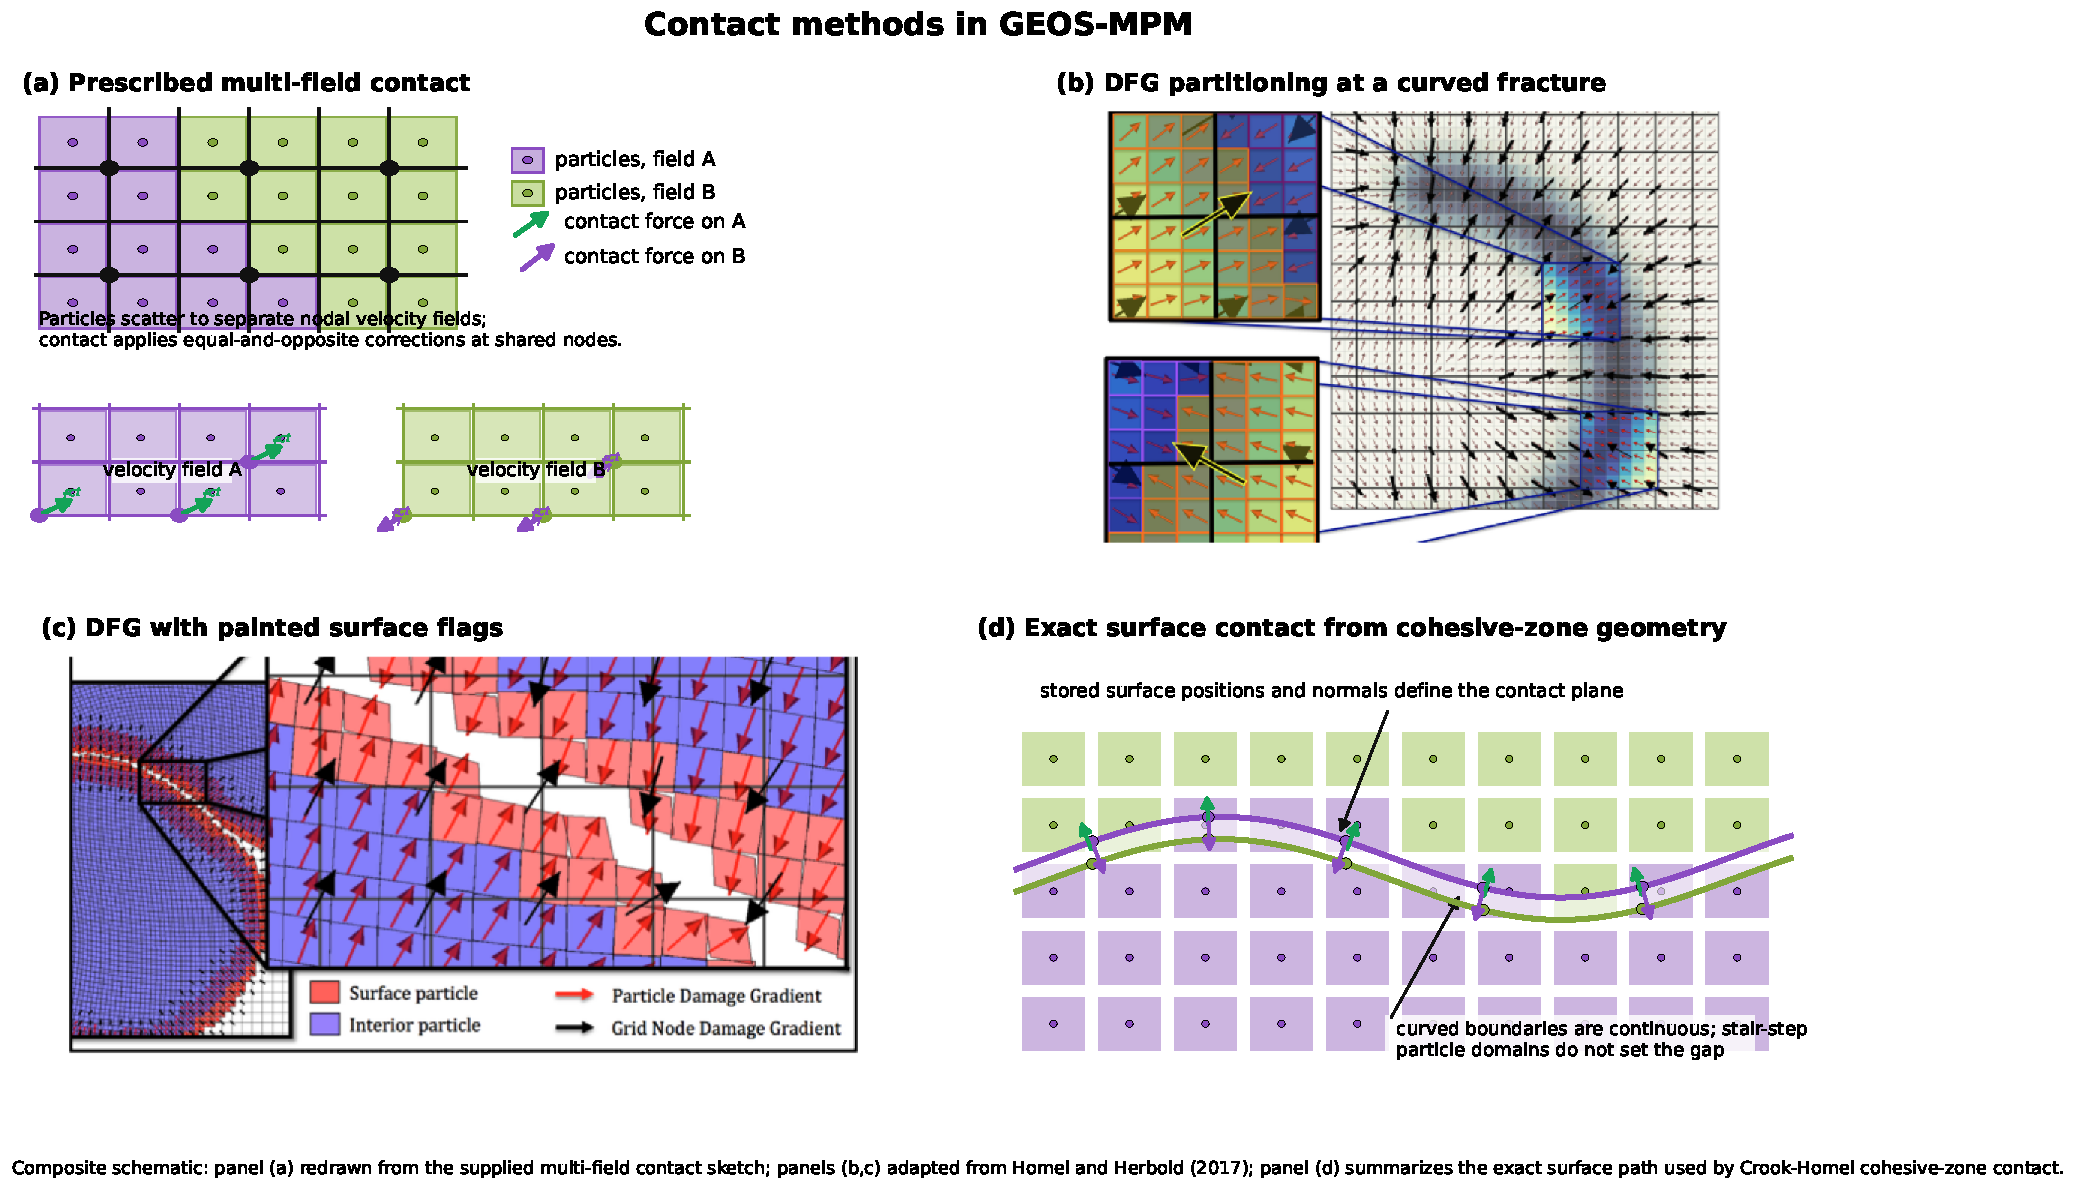
\includegraphics[width=\linewidth]{figures/contact_fields_schematic.pdf}
  \caption{Composite schematic of the contact-method families used by GEOS-MPM.  Panel (a) is redrawn from the multi-velocity-field contact concept of Bardenhagen, Guilkey, and coworkers.  Panels (b) and (c) are adapted from the DFG fracture/contact figures of Homel and Herbold.  Panel (d) summarizes the exact surface-position/normal path used by cohesive-zone-derived contact, where stored surface geometry rather than stair-step particle domains defines the gap and normal \cite{bardenhagen2001contact,homel2016dfg,crook2025cohesive}.}
  \label{fig:contact-fields-schematic}
\end{figure}

\subsection{Damage-field-gradient partitioning}
\label{subsec:dfg-contact-partitioning}
\index{DFG!partitioning}
\index{damageFieldPartitioning}

When \texttt{damageFieldPartitioning=1}, each prescribed group is split into two possible DFG flags.  The total number of nodal velocity fields becomes
\begin{equation}
  N_{\mathrm{fields}}=2N_g,
\end{equation}
with field index
\begin{equation}
  \alpha = c_p(I)N_g + g_p, \qquad c_p(I)\in\{0,1\}.
  \label{eq:dfg-field-index}
\end{equation}
The flag $c_p(I)$ is recomputed for each particle-grid mapping.  Let $\mathbf{g}_I$ be the grid damage gradient at node $I$.  Let the particle mapping normal be
\begin{equation}
  \mathbf{m}_p =
  \begin{cases}
    \nabla D_p, & \|\mathbf{n}^s_p\|\approx 0,\\
    \mathbf{n}^s_p, & \|\mathbf{n}^s_p\|>0,
  \end{cases}
\end{equation}
where $\nabla D_p$ is the particle damage gradient and $\mathbf{n}^s_p$ is the explicit particle surface normal.  The reviewed implementation assigns
\begin{equation}
  c_p(I)=
  \begin{cases}
    1, & \texttt{damageFieldPartitioning}=1\ \hbox{and}\ \mathbf{g}_I\cdot\mathbf{m}_p < 0,\\
    0, & \hbox{otherwise}.
  \end{cases}
  \label{eq:dfg-contact-flag}
\end{equation}
This sign test is the practical DFG operation: particles on opposite sides of a damage-gradient interface scatter to different velocity fields at the same node, so the solver can represent a velocity discontinuity without explicitly meshing a crack surface.

This has three important consequences.  First, DFG enables automatic self-contact for bodies with painted surface flags or evolving damage fields without requiring a priori assignment of a separate contact group to every potential contact partner.  This is especially useful in porous, fragmented, or granular configurations where the set of contacts is not known before the calculation.  Second, DFG is a kinematic enrichment for continuum damage models: once a damage band becomes sufficiently localized and passes the separability criteria, the two sides can acquire independent velocities, slip, and separation.  In this sense the method automatically inserts a contact-capable fracture surface into an otherwise continuum damage calculation.  Third, for many-body same-material problems, DFG can be cheaper than prescribed one-field-per-body contact because it requires only two DFG velocity fields per prescribed contact group, independent of how many potential same-material contacts appear within that group.

DFG and prescribed multi-field contact are compositional.  Prescribed groups determine the material or body identity $g_p$, while DFG determines the damage-side flag $c_p(I)$.  In a two-group calculation, for example, group 0 can occupy fields 0 and 2, while group 1 can occupy fields 1 and 3.  Contact between different prescribed groups is separable by construction.  Contact between the two DFG sides of the same prescribed group is allowed only when the damage and surface-quality criteria described in Section~\ref{subsec:contact-separability} are satisfied.

\subsection{Experimental weak-trace interaction with contact}
\label{subsec:contact-weak-trace-interaction}
\index{contact!weak trace projection}
\index{weak trace projection!contact interaction}

The weak-trace projection is implemented adjacent to the contact machinery because it uses the same multi-field nodal arrays and the same mapped surface-position data.  It should nevertheless be interpreted differently from contact.  Ordinary contact decides whether two fields should stick, slip, separate, or receive a compressive gap correction at a background node.  The weak-trace projection assumes a bonded weak discontinuity and enforces equality of the two field velocities at a reconstructed interface trace point,
\begin{equation}
  \mathbf{v}^{\Gamma}_{A}-\mathbf{v}^{\Gamma}_{B}=\mathbf{0},
\end{equation}
while allowing the two sides to retain independent velocity gradients.  This is intended to reduce mixed-cell stress errors at bonded material interfaces; it is not a frictional or unilateral contact model.

When \texttt{enableWeakInterfaceTraceProjection=1}, selected group pairs are identified by \texttt{weakInterfaceTracePairs}, or all prescribed group pairs are eligible if that list is empty.  If \texttt{weakInterfaceTraceSuppressNodalContact=1}, ordinary nodal contact is skipped for those pairs so that a nodal common-velocity projection does not remove the extra degrees of freedom introduced by the two fields.  This means trace coverage and trace residual diagnostics are important: if a pair is removed from ordinary nodal contact, the prescribed surface geometry and trace projection must provide the intended bonded coupling.

For prescribed trace geometry, particles on the intended bonded interface should use \texttt{SurfaceFlag::WeakDiscontinuity}.  This flag contributes explicit surface normals and positions to the grid, but it is not treated as a damage/contact surface in DFG partitioning.  By contrast, \texttt{Surface}, \texttt{FullyDamaged}, and \texttt{DamagedCohesive} remain ordinary opened or damaged surface states for contact and DFG purposes.  The weak-trace algorithm and its controls are described in Section~\ref{sec:weak-trace-implementation}; this contact section only records how that experimental branch intersects the existing contact options.

\subsection{Surface normals and surface positions}
\label{subsec:contact-surface-geometry}
\index{contact!surface normal}
\index{contact!surface position}
\index{explicitSurfaceNormalInfluence}

Each contact pair requires a normal direction and, for the more restrictive gap-closure options, a surface position.  GEOS-MPM can use explicit particle surface geometry supplied in the particle file, implicit geometry inferred from particle volume gradients, logistic-regression reconstruction from the local point cloud, or exact surface data created by cohesive-zone initialization.  The experimental weak-trace projection also consumes explicit surface positions and normals, but only to locate a bonded trace; it does not use them as a contact gap unless ordinary contact is also active for another pair.  The exact cohesive-zone path is a special case of the explicit-geometry path: the particles carry surface positions and normals tied to a smooth reference interface, so the later contact calculation can use that stored surface rather than the visible stair-step particle domain.

The grid surface normal accumulated during particle-to-grid mapping has the form
\begin{equation}
  \widetilde{\mathbf{n}}_{I\alpha}
  =\sum_{p\in\mathcal{P}_{I\alpha}} V_p\,\nabla N_{Ip}
  +\frac{\alpha}{h_{\mathrm{diag}}}
   \sum_{p\in\mathcal{P}^{s}_{I\alpha}} V_p N_{Ip}\,\mathbf{n}^{s}_p,
  \label{eq:contact-normal-scatter}
\end{equation}
where $\mathcal{P}_{I\alpha}$ is the set of particles mapped to node $I$ and field $\alpha$, $\mathcal{P}^{s}_{I\alpha}$ is the subset with explicit surface normals, and $\alpha=\texttt{explicitSurfaceNormalInfluence}$ is dimensionless.  The grid metric is the active cell diagonal,
\begin{equation}
  h_{\mathrm{diag}}=
  \begin{cases}
    \sqrt{h_x^2+h_y^2}, & \text{plane strain},\\
    \sqrt{h_x^2+h_y^2+h_z^2}, & \text{three dimensions}.
  \end{cases}
\end{equation}
The first term is the implicit volume-gradient normal used by DFG-style surface reconstruction.  The second term lets explicitly supplied particle surface normals dominate the grid normal when the dimensionless influence factor is chosen large enough.  Dividing by $h_{\mathrm{diag}}$ makes this explicit contribution scale like $V_p\nabla N_{Ip}$, so the relative weighting is independent of the model's physical length scale and of uniform mesh refinement.  The scale is computed from the grid spacing, not from partition-local nodal sums, so the treatment does not introduce a new decomposition-dependent threshold.  The normalized vector is
\begin{equation}
  \hat{\mathbf{n}}_{I\alpha}=\frac{\widetilde{\mathbf{n}}_{I\alpha}}{\|\widetilde{\mathbf{n}}_{I\alpha}\|},
\end{equation}
with the $z$ component removed in plane-strain calculations.

When a particle has an explicit surface normal and surface position, the solver also scatters a nodal surface-position vector.  The scalar signed distance from node $I$ to the particle surface along the particle normal is
\begin{equation}
  s_{Ip}=\left(\mathbf{x}^{s}_p+\mathbf{x}_p-\mathbf{x}_I\right)\cdot\mathbf{n}^{s}_p.
\end{equation}
The corresponding grid contribution is
\begin{equation}
  \mathbf{x}^{s}_{I\alpha}
  \leftarrow
  \mathbf{x}^{s}_{I\alpha}
  +m_p N_{Ip}\,s_{Ip}\,\mathbf{n}^{s}_p,
  \label{eq:contact-surface-position-scatter}
\end{equation}
with a separate mass-like normalization stored in \texttt{gridSurfaceFieldMass}.  When \texttt{useSurfacePositionForContact=1}, these surface positions are used by the gap criterion if both fields have sufficient surface-position mass; otherwise the contact law falls back to field centers with a spacing correction.

\begin{figure}[htbp]
  \centering
  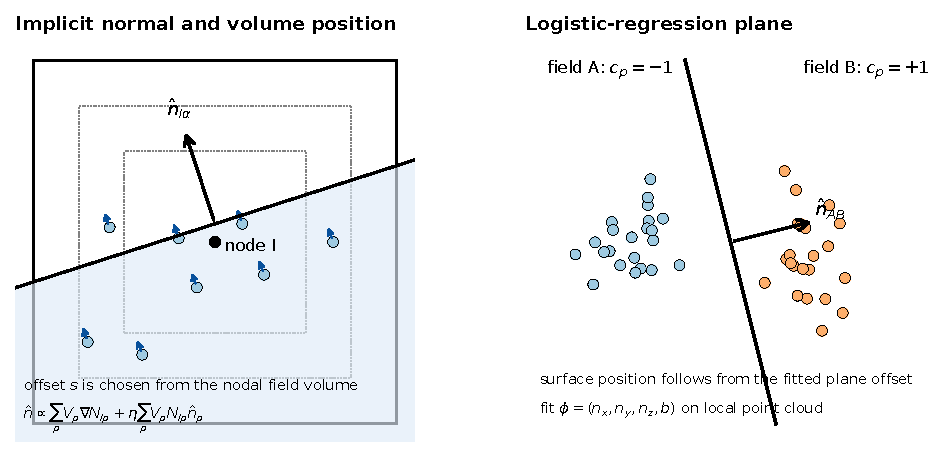
\includegraphics[width=0.96\linewidth]{figures/contact_surface_methods_schematic.pdf}
  \caption{Schematic of the two automatic surface-geometry families.  Left: an implicit normal from mapped particle volume gradients, optionally biased by explicit particle normals, plus a volume-matched plane position.  Right: a logistic-regression plane fitted to the two local field point clouds.  The figure is newly drawn for this manual and is conceptually adapted from DFG and regression-based MPM contact descriptions \cite{homel2016dfg,nairn2020contact}.}
  \label{fig:contact-surface-methods}
\end{figure}

\subsection{Automatic particle normal and position reconstruction}
\label{subsec:automatic-surface-reconstruction}
\index{computeParticleSurfaceNormalsAndPositions}
\index{normalAndPositionMethod}

The option \texttt{computeParticleSurfaceNormalsAndPositions} invokes a one-time reconstruction pass before the particle-to-grid stage of the step in which the flag is seen.  The pass first scatters temporary mass, volume, and the raw normal in Eq.~\eqref{eq:contact-normal-scatter}.  It then branches on \texttt{normalAndPositionMethod}:
\begin{description}
  \item[\texttt{DFGAndVolumeIntegration}.] The normalized DFG or volume-gradient normal is kept as the grid-based normal.  The grid-based surface position is recovered by matching the mapped nodal field volume to the volume of a weighted half-space, as described in Section~\ref{subsec:volume-method-contact-position}.
  \item[\texttt{LogisticRegression}.] For each active node and each active field pair, the solver fits a plane to the local two-field point cloud, stores opposite normals and offsets for the two fields, and then maps those normals and positions back to the particles.
\end{description}
After either branch, \texttt{mapSurfaceNormalsAndPositionsToParticles} transfers the reconstructed geometry back to particle fields and updates the corresponding reference normal and reference surface-position fields.  The temporary grid mass, volume, and surface-normal arrays used by the reconstruction are zeroed at the end of the pass so that subsequent particle-to-grid operations start from a clean state.

\subsection{Logistic-regression surface reconstruction}
\label{subsec:logistic-regression-contact-normal}
\index{contact!logistic regression}
\index{LogisticRegression}

The logistic-regression method follows the point-cloud philosophy described by Nairn, Hammerquist, and Smith: rather than deriving the interface solely from grid data, it estimates the most probable local plane separating two material point clouds at a contact node \cite{nairn2020contact}.  For a node $I$ and field pair $(A,B)$, the reviewed implementation constructs feature vectors
\begin{equation}
  \boldsymbol{\xi}_p=\begin{bmatrix}
  x_{p,1}-x_{I,1} & x_{p,2}-x_{I,2} & x_{p,3}-x_{I,3} & 1
  \end{bmatrix}^{T},
\end{equation}
using neighboring particles that partition into either field $A$ or field $B$.  The class label is
\begin{equation}
  c_p=\begin{cases}
  -1, & p\mapsto A,\\
  +1, & p\mapsto B.
  \end{cases}
\end{equation}
For parameter vector $\boldsymbol{\phi}=(n_1,n_2,n_3,b)^T$, the code uses the logistic score
\begin{equation}
  \widehat{c}_p(\boldsymbol{\phi})=\frac{2}{1+\exp(-\boldsymbol{\xi}_p\cdot\boldsymbol{\phi})}-1.
\end{equation}
The nonlinear least-squares update is regularized on the normal components,
\begin{equation}
  \min_{\boldsymbol{\phi}}
  \sum_{p} w_p\left(c_p-\widehat{c}_p(\boldsymbol{\phi})\right)^2
  +\lambda\left(n_1^2+n_2^2+n_3^2\right),
  \label{eq:contact-logistic-objective}
\end{equation}
with $w_p=1$ and $\lambda=10^{-7}\|\mathbf{h}\|^2$ in the reviewed code.  The initial normal is the mass-weighted pair normal, $m_A\mathbf{n}_A-m_B\mathbf{n}_B$.  Iteration stops when the normalized surface-position change is below \texttt{LRtolerance}, or when \texttt{maxLRIterations} is reached.  If the local $4\times4$ matrix is singular or the normal magnitude collapses, the code falls back to the previous normal and surface position.

The fitted normal is the normalized first three components of $\boldsymbol{\phi}$.  The implemented surface offset is
\begin{equation}
  s=\frac{-\log(1/3)-b}{\|\mathbf{n}\|},
  \qquad
  \mathbf{x}^{s}_{I,AB}=s\,\hat{\mathbf{n}}_{AB}.
  \label{eq:contact-lr-offset}
\end{equation}
This is used both as an automatic surface-position reconstruction option and, when the requested pair normal type is \texttt{LogisticRegression}, as an on-demand pair-normal calculation inside the contact loop.

\subsection{Volume method for contact surface position}
\label{subsec:volume-method-contact-position}
\index{contact!volume position}
\index{DFGAndVolumeIntegration}

The \texttt{DFGAndVolumeIntegration} position method assumes that a partially filled nodal support can be approximated by a fully dense half-space cut by a plane with known unit normal $\hat{\mathbf{n}}_{I\alpha}$.  The unknown is the plane offset $s$ from the grid node.  Let $\mathbf{r}=\mathbf{x}-\mathbf{x}_I$ and define the trilinear support weight
\begin{equation}
  W_I(\mathbf{r})=
  \left(1-\frac{|r_1|}{h_1}\right)
  \left(1-\frac{|r_2|}{h_2}\right)
  \left(1-\frac{|r_3|}{h_3}\right)
\end{equation}
inside the nodal support and zero outside.  The volume predicted by an offset $s$ is
\begin{equation}
  \mathcal{V}(s)=
  \int_{\mathrm{supp}(I)}
  H\!\left(s-\hat{\mathbf{n}}_{I\alpha}\cdot\mathbf{r}\right)
  W_I(\mathbf{r})\,dV.
  \label{eq:contact-volume-offset}
\end{equation}
The solver performs bisection over the admissible offset interval and chooses $s$ such that $\mathcal{V}(s)$ matches the mapped grid material volume $V_{I\alpha}$ to a tolerance of $10^{-3}$ cell volumes.  The numerical integration currently uses a structured $200^3$ quadrature over the nodal support.  Cells with zero mapped volume and cells with mapped volume greater than or equal to the cell volume are ignored; the latter limitation matters when contact overlap or densification produces overfilled nodal supports.

\subsection{Pair-normal weighting between fields}
\label{subsec:contact-normal-weighting}
\index{contactNormalType}
\index{contact!normal weighting}

The field normals $\mathbf{n}_A$ and $\mathbf{n}_B$ must be reduced to a single pair normal $\hat{\mathbf{n}}_{AB}$ oriented outward from field $A$ toward field $B$.  GEOS-MPM exposes the following \texttt{contactNormalType} branches:

\begin{longtable}{p{0.27\linewidth}p{0.66\linewidth}}
\toprule
Option & Solver operation \\
\midrule
\endhead
\texttt{Difference} & Uses $\mathbf{n}_{AB}=\mathbf{n}_A-\mathbf{n}_B$ before normalization.  This is the simplest symmetric difference of the two outward normals. \\
\texttt{MassWeighted} & Uses $\mathbf{n}_{AB}=m_A\mathbf{n}_A-m_B\mathbf{n}_B$.  This is the constructor default in the reviewed source. \\
\texttt{LargerMass} & Uses $\mathbf{n}_A$ if $m_A>m_B$, otherwise uses $-\mathbf{n}_B$.  This can be useful when a heavy or well-resolved field should dominate the pair normal. \\
\texttt{Mixed} & Compares field densities $\rho_A=m_A/V_A$ and $\rho_B=m_B/V_B$.  If they are similar, it uses the mass-weighted normal.  Otherwise it uses the normal of the denser field. \\
\texttt{Aligned} & Uses explicit-normal alignment weights to suppress poorly aligned field normals.  The current code computes a smoothstep weight above a fixed threshold of 0.9 and forms the weighted difference.  The attribute \texttt{contactNormalExponent} is registered, but the active branch uses the fixed smoothstep weighting rather than the commented exponentiation lines. \\
\texttt{LogisticRegression} & Re-fits a logistic-regression plane for the specific field pair at the contact node and uses the fitted plane normal as $\mathbf{n}_{AB}$. \\
\bottomrule
\end{longtable}

For the \texttt{Aligned} option, the alignment weights are accumulated during particle-to-grid mapping from particles with explicit normals.  In abstract notation, the weight is a mass-normalized average of the particle/grid normal agreement,
\begin{equation}
  w_{I\alpha}=\frac{\sum_{p\in\mathcal{P}^{s}_{I\alpha}} m_pN_{Ip}\,
  \left(\hat{\mathbf{n}}_{I\alpha}\cdot\hat{\mathbf{n}}^s_p\right)}
  {\sum_{p\in\mathcal{P}^{s}_{I\alpha}} m_pN_{Ip}}.
\end{equation}
The pair normal is normalized after the option-specific construction, and the solver stores opposite normals back to the two grid fields for consistency.

\subsection{Separability criteria}
\label{subsec:contact-separability}
\index{contact!separability}
\index{separabilityMinDamage}
\index{surfaceQualityThreshold}
\index{thinFeatureDFGThreshold}

The contact law first decides whether two fields are bonded together at the node or represent separable surfaces.  If they are not separable, the nodal correction drives both fields toward the center-of-mass velocity in both normal and tangential directions, which is effectively a no-slip compatibility correction.  If they are separable, the normal and Coulomb-like tangential contact law is applied only when the gap-closure criterion is satisfied.

The separability criterion is
\begin{equation}
\begin{aligned}
  \mathrm{separable} ={}&
  \Big[\big(\max(D_A^{\max},D_B^{\max})\ge 0.9999\big)
  \land \big(D_A\ge D_{\min}\big) \\
  &\qquad {}
  \land \big(D_B\ge D_{\min}\big)
  \land \big(Q_s\ge Q_{\min}\big)\Big] \\
  &{}\lor \big(A\bmod N_g\ne B\bmod N_g\big),
  \label{eq:contact-separability}
\end{aligned}
\end{equation}
where $D_{\min}=\texttt{separabilityMinDamage}$ and $Q_{\min}=\texttt{surfaceQualityThreshold}$.  The second term means that different prescribed contact groups are separable regardless of damage.  The first term is the same-group DFG/fracture branch: at least one field must be essentially fully damaged, both fields must exceed the minimum damage threshold, and the local mapping-normal tensor quality must meet the configured threshold.

For each particle-node contribution, the mapping normal $\hat{\mathbf{m}}_p$ is the same normal used by the DFG partitioner: the normalized explicit particle surface normal when that normal is present, otherwise the normalized particle damage gradient.  The grid stores a sign-invariant orientation tensor for each velocity field,
\begin{equation}
  \mathbf{M}_{I\alpha} = \sum_{p\in\mathcal{P}_{I\alpha}} V_p N_{Ip}\,
  \hat{\mathbf{m}}_p\otimes\hat{\mathbf{m}}_p,
  \label{eq:dfg-mapping-normal-tensor}
\end{equation}
with components stored as \texttt{gridMappingNormalTensor}.  For a pair of fields, $\mathbf{M}_{AB}=\mathbf{M}_{IA}+\mathbf{M}_{IB}$.  Let $d=2$ in plane strain and $d=3$ otherwise, let $\lambda_{\max}$ be the largest eigenvalue of $\mathbf{M}_{AB}$ over the active dimensions, and let $T=\mathrm{tr}(\mathbf{M}_{AB})$ over those same dimensions.  The surface quality is
\begin{equation}
  Q_s =
  \min\!\left(1,\frac{T}{V_{IA}+V_{IB}}\right)
  \frac{d\lambda_{\max}/T-1}{d-1},
  \qquad 0\le Q_s\le 1.
  \label{eq:dfg-surface-quality}
\end{equation}
It is one when the mapped material volume is fully covered by one coherent normal axis, including anti-parallel crack-face normals, and it is zero when the valid mapping normals do not define a preferred axis or no valid mapping normal contributes.

Two additional guards can suppress separability.  If \texttt{maxSingleFieldStateFractionForSeparability} is nonnegative, the code maps the volume-weighted fraction of particles that are fully damaged, melted, or domain-reset to each grid field and treats a field pair as inseparable when the pair-average fraction exceeds the configured value.  A value of 0.999 preserves the legacy intent of suppressing separability only in essentially fully single-field regions.  If \texttt{thinFeatureDFGThreshold} is set below its large default value, a DFG pair with very small field-center spacing relative to the neighbor radius is also forced to be inseparable.  The thin-feature guard uses
\begin{equation}
  \|\mathbf{x}_A-\mathbf{x}_B\|^2 <
  \big(\texttt{thinFeatureDFGThreshold}\,r_n\big)^2,
  \label{eq:dfg-thin-feature-guard}
\end{equation}
where $r_n$ is the neighbor radius.  This prevents a thin strip of material, whose two physical surfaces are closer than the grid resolution, from being spuriously split into internal slip surfaces.

\subsection{Gap closure and frictional contact}
\label{subsec:contact-gap-closure}
\index{contactGapCorrection}
\index{contact!gap closure}
\index{contact!friction}

For a field pair, the center-of-mass velocity is
\begin{equation}
  \mathbf{v}_{AB}=\frac{\mathbf{q}_A+\mathbf{q}_B}{m_A+m_B}.
\end{equation}
The normal correction needed to bring field $A$ to the center-of-mass normal velocity is proportional to
\begin{equation}
  f_n=\frac{m_A}{\Delta t}\left(\mathbf{v}_{AB}-\mathbf{v}_A\right)\cdot\hat{\mathbf{n}}_{AB}
  \label{eq:contact-normal-force-core}
\end{equation}
for the force form, or to the same expression without $1/\Delta t$ for the impulse form.  The solver uses an orthonormal basis $\{\hat{\mathbf{n}}_{AB},\hat{\mathbf{s}}_1,\hat{\mathbf{s}}_2\}$ to compute tangential sticking forces or impulses.  For separable contact, the normal force is multiplied by a gap-closure factor $\chi\in[0,1]$, and the tangential force magnitude is limited by
\begin{equation}
  |f_t|\le \mu_{AB}|f_n|.
\end{equation}
If cohesive tangential forces are active for the pair, the frictional tangential contribution is set to zero so that the cohesive law supplies the tangential resistance.

The gap length scale used by the contact criterion is the grid-normal support length,
\begin{equation}
  g_0 = \left(\sum_{i=1}^{d}\frac{\hat n_{AB,i}^{2}}{h_i^2}\right)^{-1/2},
  \label{eq:contact-gap0}
\end{equation}
with $d=2$ for plane strain and $d=3$ otherwise.  If both fields have usable surface positions and \texttt{useSurfacePositionForContact=1}, the solver uses those positions in the gap,
\begin{equation}
  g=(\mathbf{x}^{s}_B-\mathbf{x}^{s}_A)\cdot\hat{\mathbf{n}}_{AB}.
\end{equation}
If one or both fields lack surface positions, the corresponding field center is used and the code subtracts $0.5g_0$ for each missing side.  In the general implemented form,
\begin{equation}
  g=(\mathbf{x}^{*}_B-\mathbf{x}^{*}_A)\cdot\hat{\mathbf{n}}_{AB}-\gamma g_0,
  \qquad \gamma\in\{0,0.5,1\},
  \label{eq:contact-gap-general}
\end{equation}
where $\mathbf{x}^{*}$ is either a surface position or a field center.

The approach test is
\begin{equation}
  a=(\mathbf{v}_A-\mathbf{v}_{AB})\cdot\hat{\mathbf{n}}_{AB}.
\end{equation}
The \texttt{contactGapCorrection} option selects the closure factor:
\begin{equation}
\chi =
\begin{cases}
  H(a), & \texttt{Simple},\\
  H(a)H(-g), & \texttt{Implicit},\\
  H(a), & \texttt{Softened}\ \hbox{and}\ g\le 0,\\
  H(a)\left(1-g/g_0\right), & \texttt{Softened}\ \hbox{and}\ 0<g<g_0,\\
  0, & \texttt{Softened}\ \hbox{and}\ g\ge g_0,
\end{cases}
\label{eq:contact-gap-closure-factor}
\end{equation}
where $H$ is the Heaviside step function.  \texttt{Simple} is purely velocity based and can close gaps before geometric overlap is detected.  \texttt{Implicit}, the current default, requires both approach and negative gap.  \texttt{Softened} ramps the normal correction over one grid-normal support length to avoid a discontinuous on/off transition near first contact.

\subsection{Global and group-dependent friction coefficients}
\label{subsec:contact-friction-coefficients}
\index{frictionCoefficient}
\index{frictionCoefficientTable}
\index{contact!friction table}

The tangential contact limit uses a coefficient $\mu_{AB}$ chosen from a solver-side square table.  The contact loop does not distinguish whether the table was supplied directly or expanded from a scalar; it simply evaluates
\begin{equation}
  \mu_{AB}=\texttt{frictionCoefficientTable}
  \left[A\bmod N_g,\,B\bmod N_g\right],
  \label{eq:contact-friction-table-index}
\end{equation}
where $A$ and $B$ are velocity-field indices and $N_g$ is the number of prescribed contact groups.  The modulo reduction is important when DFG is active: the DFG side flag changes the velocity-field index, but the friction lookup still refers to the underlying prescribed group.

If the input provides only the scalar \texttt{frictionCoefficient}, \texttt{initializeFrictionCoefficients} expands it to a uniform $N_g\times N_g$ table,
\begin{equation}
  \mu_{ij}=\mu_{\mathrm{global}},\qquad i,j=0,\ldots,N_g-1.
\end{equation}
A scalar value of \texttt{-1} is interpreted as unspecified and is converted to zero friction before the table is built; negative values after that conversion are rejected.  This global mode is concise for homogeneous interfaces, DFG self-contact with a single material, and verification problems where all material pairs should share the same Coulomb limit.

If \texttt{frictionCoefficientTable} is supplied, it is used directly after validation.  The table must be square, its number of rows and columns must equal $N_g$, and off-diagonal entries must be symmetric.  Off-diagonal entries control prescribed group-group interfaces, while diagonal entries control same-group contact, including DFG self-contact or post-failure contact between the two sides of a same-group fracture.  A \texttt{FrictionCoefficientSwap} event can later replace either the scalar coefficient or the table; after the event the same initialization logic is called, so the material contact loop always sees a validated table.

\subsection{Overdensification and overlap correction}
\label{subsec:overdensification-overlap-correction}
\index{overlapCorrection}
\index{overlapThreshold1}
\index{overlapThreshold2}
\index{computeSPHJacobian}
\index{directionalOverlapCorrection}

Contact, DFG, CPDI domain changes, and high compression can create nodal or particle states that are too dense relative to the grid or to a nonlocal particle-volume estimate.  GEOS-MPM provides several overlap-control branches.  These should be viewed as stabilization or correction options rather than replacements for a well-resolved contact surface.

\begin{description}
  \item[\texttt{Off}.] No additional overlap correction is applied beyond the contact law.

  \item[\texttt{NormalForce}.] During pairwise nodal contact, the code estimates an overlap length from the sum of the pair volumes and the grid support geometry.  In 3D,
  \begin{equation}
    \ell_{\mathrm{ov}}=\frac{V_A+V_B-V_{\mathrm{cell}}}{A_{\perp}},
    \qquad
    A_{\perp}=\frac{V_{\mathrm{cell}}}{\sum_i |\hat n_i|h_i}.
  \end{equation}
  In plane strain the implementation uses the corresponding half-cell support convention.  If $\ell_{\mathrm{ov}}$ lies between the two threshold levels \texttt{overlapThreshold1} and \texttt{overlapThreshold2}, an additional compressive normal force or impulse is added.  The correction is ramped from zero to full strength across the threshold interval and is limited by a CFL-like velocity bound proportional to $0.05\min(m_A,m_B)v_{\max}/\Delta t$ in force form.

  \item[\texttt{SPH}.] Post-input initialization forces \texttt{computeSPHJacobian=1}.  Each step computes a nonlocal SPH estimate of the particle Jacobian, $J_{\mathrm{SPH}}$, from neighboring particles.  After the standard deformation-gradient update, the correction compares the constitutive-particle Jacobian $J=\det\mathbf{F}$ to the nonlocal value through
  \begin{equation}
    r=\frac{J}{J_{\mathrm{SPH}}}.
  \end{equation}
  If $r>\texttt{overlapThreshold1}$, a smoothstep ramp toward the SPH Jacobian is applied.  The deformation gradient is scaled by
  \begin{equation}
    s=\begin{cases}
      \left(1+\alpha(r^{-1}-1)\right)^{1/2}, & \hbox{plane strain},\\
      \left(1+\alpha(r^{-1}-1)\right)^{1/3}, & \hbox{3D},
    \end{cases}
  \end{equation}
  with $s\ge0.99$ so the density correction cannot change too much in a single step.  The code also updates \texttt{particleFDot} and adjusts the velocity gradient consistently with the scaled deformation gradient.  Comments in the source note that the SPH estimate can be noisy near free and symmetry boundaries.

  \item[\texttt{Volume}.] During grid-to-particle transfer, the solver estimates the nodal material volume divided by the nodal support volume.  If this overlap measure exceeds \texttt{overlapThreshold1}, the diagonal particle velocity-gradient components are reduced by a small compressive correction proportional to $(\mathrm{overlap}-1)/\Delta t$.  The current implementation is deliberately gentle, targeting roughly a 100-step correction time.  Because the reviewed code sums a group-indexed subset of grid material volumes in this branch, DFG multi-flag cases should be verified before using \texttt{Volume} as the primary overlap-control mechanism.
\end{description}

The separate flag \texttt{directionalOverlapCorrection} registers a particle \texttt{particleSPHF} tensor and activates neighbor-list construction.  The reviewed source also contains a kernel-based \texttt{computeSphF} helper that estimates a deformation-like tensor from reference and current neighbor positions.  In the current explicit-step sequence, however, this directional path is not wired into the main overlap-correction loop in the same way as \texttt{SPH}, \texttt{Volume}, and \texttt{NormalForce}.  Treat it as a development hook unless a dedicated verification case exercises it.


\subsection{Summary examples and verification targets}
\label{subsec:contact-summary-examples}
\index{contact!examples}
\index{DFG!large deformation contact}
\index{cohesive zone!explicit surface contact}

The contact options above can be viewed as a hierarchy of increasingly geometric contact descriptions.  Prescribed multi-field contact supplies the velocity fields directly through particle groups.  DFG supplies the velocity-field split dynamically from the damage-gradient or painted surface data.  Logistic regression reconstructs a local separating surface from the two-field point cloud.  The cohesive-zone surface path supplies exact surface positions and normals from the initialized cohesive interface and therefore keeps curved contact geometry independent of the stair-step outline of the particle domains.  Verification should exercise each of these descriptions separately and in combination with FMPM, boundary motion, frictional slip, gap closure, and overdensification control.

Figure~\ref{fig:contact-examples-summary} records two representative high-value verification targets.  The first is the large-deformation DFG contact example represented by Fig.~9 of Homel and Herbold's field-gradient partitioning paper, where a dynamically evolving damage/fracture surface must split the material into contact-capable sides without pre-defining every potential contact pair \cite{homel2016dfg}.  The second is indentation against an explicitly described surface from the Crook-Homel cohesive-zone formulation.  In that case, the relevant contact test is not merely that particles do not interpenetrate; it is that the gap, normal, and tangential slip response remain controlled by the stored smooth surface positions and normals after a cohesive interface transitions into ordinary contact \cite{crook2025cohesive}.

\begin{figure}[htbp]
  \centering
  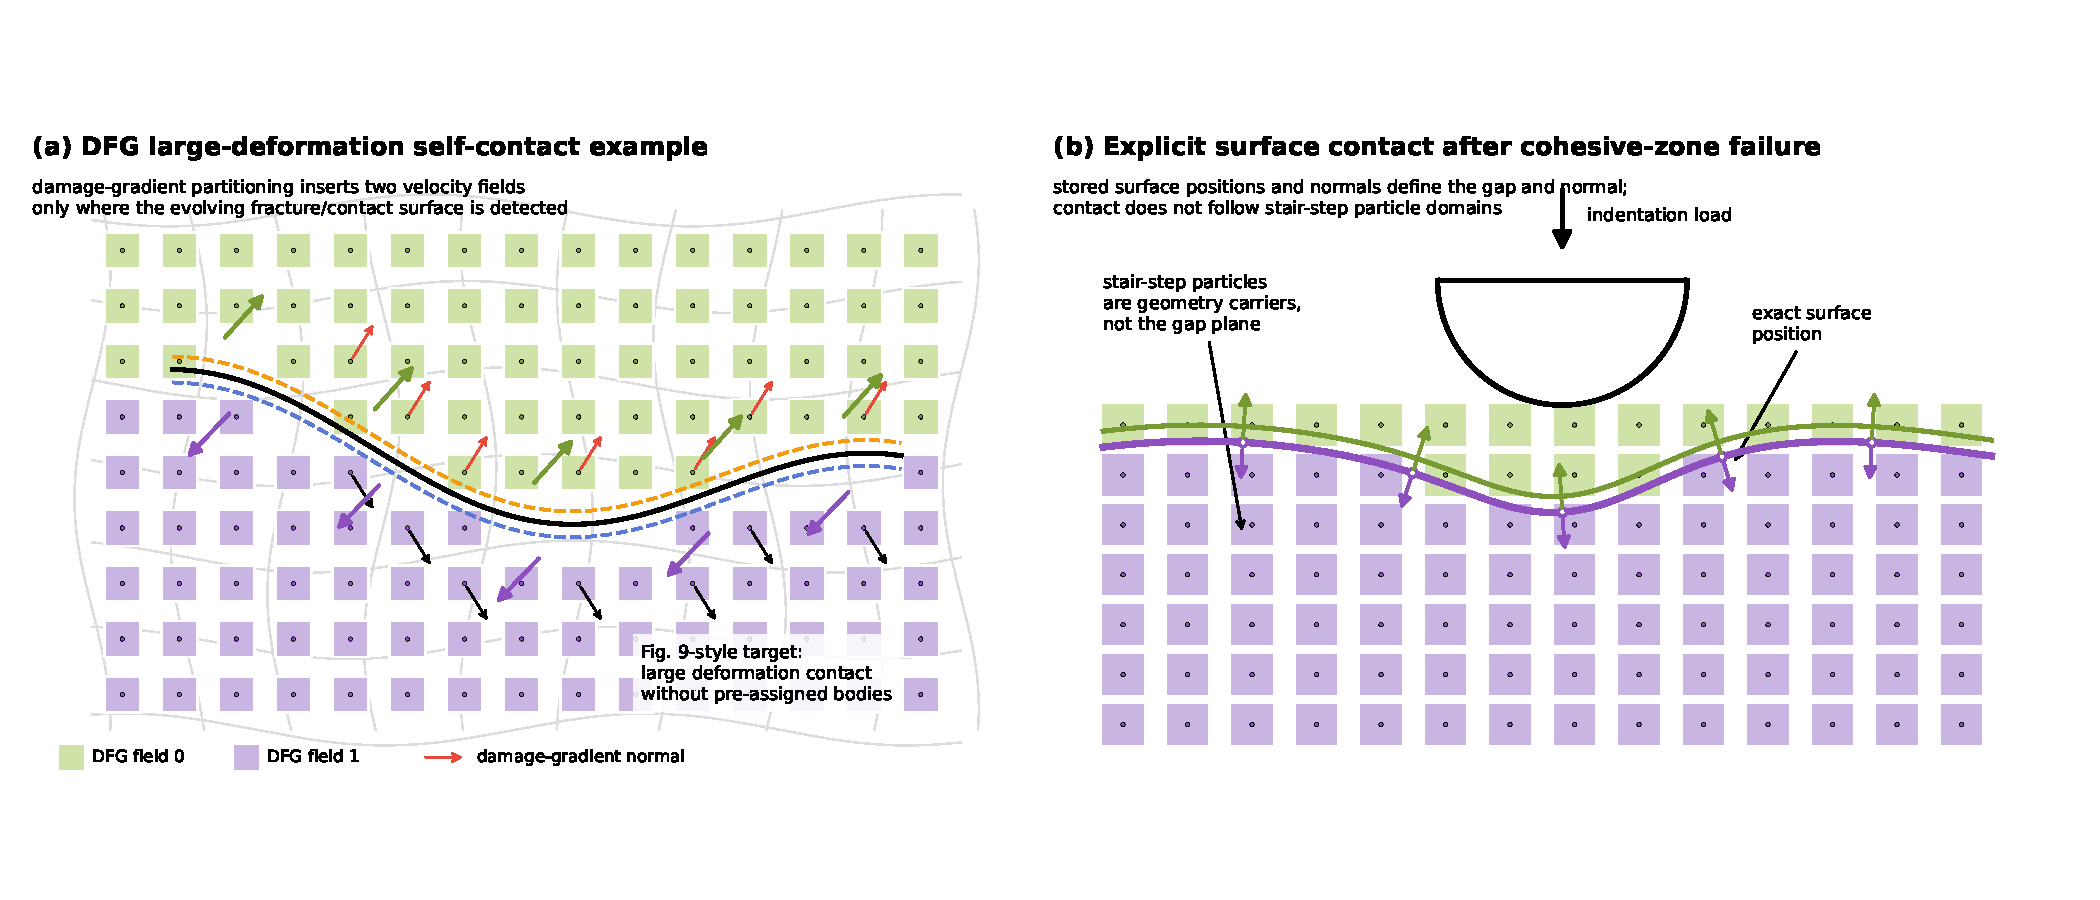
\includegraphics[width=\linewidth]{figures/contact_examples_summary.pdf}
  \caption{Representative contact verification targets.  Panel (a) is an original schematic inspired by the large-deformation DFG contact demonstration, Fig.~9 of Homel and Herbold \cite{homel2016dfg}.  Panel (b) is an original schematic inspired by the indentation/explicit-surface contact capability in the Crook-Homel cohesive-zone formulation \cite{crook2025cohesive}.}
  \label{fig:contact-examples-summary}
\end{figure}

A useful verification matrix is: (i) prescribed two-body contact with a scalar global friction coefficient, (ii) prescribed multi-body contact with a symmetric group-dependent friction table, (iii) DFG same-material self-contact with a nonzero diagonal friction entry, (iv) DFG plus prescribed groups where field indices use the modulo friction-table lookup, (v) logistic-regression contact on a curved or oblique two-material interface, (vi) cohesive-zone-derived exact surface contact after cohesive failure, (vii) prescribed weak-trace projection on a bonded two-material interface, and (viii) each contact case under \texttt{Simple}, \texttt{Implicit}, and \texttt{Softened} gap closure.  Overlap correction should then be tested as an optional stabilization layer rather than as the primary mechanism for enforcing contact.  The weak-trace case should be judged primarily by local mixed-cell stress error and trace velocity residuals, not only by global stress--strain response.

\subsection{Input controls and cross references}
\label{subsec:contact-input-summary-theory}
\index{contact!input summary}

Table~\ref{tab:contact-input-summary-theory} summarizes the solver attributes most directly tied to the contact algorithms above.  These are solver-side controls.  Section~\ref{sec:pfw-boundary-controls} should describe how PFW exposes or forwards them from \texttt{pfw\_input}, and Appendix~\ref{app:solver-attributes} provides the generated attribute inventory.

\begingroup\small
\begin{longtable}{>{\raggedright\arraybackslash}p{0.36\linewidth}>{\raggedright\arraybackslash}p{0.56\linewidth}}
\caption{Internal contact controls discussed in Section~\ref{sec:contact-options}.}\label{tab:contact-input-summary-theory}\\
\toprule
Attribute & Internal effect \\
\midrule
\endfirsthead
\toprule
Attribute & Internal effect \\
\midrule
\endhead
\texttt{enableContact} & Master switch for material contact once \texttt{hasContact} is true. \\
\texttt{damageFieldPartitioning} & Enables DFG two-flag splitting inside each prescribed contact group. \\
\texttt{contactNormalType} & Selects the pair-normal construction branch: \texttt{Difference}, \texttt{MassWeighted}, \texttt{LargerMass}, \texttt{Mixed}, \texttt{Aligned}, or \texttt{LogisticRegression}. \\
\texttt{contactGapCorrection} & Selects \texttt{Simple}, \texttt{Implicit}, or \texttt{Softened} closure in Eq.~\eqref{eq:contact-gap-closure-factor}. \\
\texttt{frictionCoefficient} & Scalar global coefficient expanded to a uniform group-group table when no explicit table is supplied. \\
\texttt{frictionCoefficientTable} & Defines pairwise group-dependent friction coefficients; must be square, must match the number of contact groups, and is indexed by $A\bmod N_g$ and $B\bmod N_g$ when DFG adds fields. \\
\begin{tabular}[t]{@{}l@{}}\texttt{computeParticleSurface}\\\texttt{NormalsAndPositions}\end{tabular} & Triggers automatic particle normal/position reconstruction. \\
\texttt{normalAndPositionMethod} & Chooses \texttt{LogisticRegression} or \texttt{DFGAndVolumeIntegration} for automatic reconstruction. \\
\texttt{explicitSurfaceNormalInfluence} & Dimensionless control for the relative strength of explicit particle normals in the grid normal scatter; internally divided by the active grid-cell diagonal. \\
\texttt{useSurfacePositionForContact} & Allows surface-position fields to replace center-of-volume positions in the gap calculation when available. \\
\texttt{LRtolerance}, \texttt{maxLRIterations} & Control convergence and iteration limit of the logistic-regression fit. \\
\texttt{surfaceQualityThreshold}, \texttt{separabilityMinDamage} & Control same-group DFG separability; the surface-quality threshold is applied to the mapping-normal orientation tensor. \\
\texttt{thinFeatureDFGThreshold} & Suppresses separability for DFG pairs whose field centers are closer than the configured fraction of the neighbor radius. \\
\texttt{maxSingleFieldStateFractionForSeparability} & Suppresses separability when the mapped fully damaged, melted, or domain-reset particle fraction exceeds the configured value. \\
\texttt{overlapCorrection} & Selects \texttt{Off}, \texttt{NormalForce}, \texttt{SPH}, or \texttt{Volume}. \\
\texttt{overlapThreshold1}, \texttt{overlapThreshold2} & Define ramp thresholds for overlap-correction branches. \\
\texttt{computeSPHJacobian} & Computes nonlocal SPH Jacobian data; automatically enabled by \texttt{overlapCorrection=SPH}. \\
\texttt{directionalOverlapCorrection} & Development hook for neighbor-based directional overlap data. \\
\texttt{enableWeakInterfaceTraceProjection} & Experimental bonded trace projection between selected velocity-field pairs; see Section~\ref{sec:weak-trace-implementation}. \\
\texttt{weakInterfaceTracePairs} & Optional group-pair list for the weak-trace branch.  Empty means all group pairs are eligible. \\
\texttt{weakInterfaceTraceProjectionScale}, \texttt{weakInterfaceTraceProjectionIterations} & Under-relaxation and local iteration count for the weak-trace projection. \\
\texttt{weakInterfaceTraceGapStabilization}, \texttt{weakInterfaceTraceMinWeight} & Optional trace drift stabilization and minimum active trace support. \\
\texttt{weakInterfaceTraceSuppressNodalContact} & Suppresses ordinary nodal contact for pairs handled by the experimental weak-trace branch. \\
\bottomrule
\end{longtable}
\endgroup
